% Chapter Template

\chapter{Numerical Investigation and Discussion} % Main chapter title

\label{Chapter6} % Change X to a consecutive number; for referencing this chapter elsewhere, use \ref{ChapterX}

This chapter will empirically compare the numerical and analytical methods presented for different types of contingent claims\footnote{The interested reader can see the implementation details in appendix \ref{AppendixD}}. The underlying model will be the Black-Scholes model, because it has closed form solutions for some European options and is thoroughly researched.\\

We look at the closed form solutions to the European options compared with the binomial lattice model for pricing. The closed form solution provides a measure of how the binomial lattice model approximates European options in the Black-Scholes model. The binomial model is readily extended to American options, hence, the section also gives an indication of how the binomial model approximates the American option. The American put option is then investigated, where the different numerical methods considered are compared. The last type of option we look at is the American put minimum on two stocks option. After the numerical investigation, the pricing methods and model assumptions are discussed.


%----------------------------------------------------------------------------------------
%	SECTION 1
%----------------------------------------------------------------------------------------
\section{European Options}\label{EuroOption}
European options are simple in the sense that they can only be exercised at maturity. Throughout the previous chapters, especially chapter \ref{Chapter2} and \ref{Chapter3}, we have seen closed form solutions for the simple European and exotic European options. The binomial lattice models presented are models that can approximate European options and American options. The closed form solutions and the binomial lattice approach can be compared for European options, where a small deviation between methods for the European options indicates that the lattice approach gives reasonable prices for the American options.\\

The simplest case is the European call option, where we look at how the CRR model and the MLP II pricing model approximate the B-S call formula. Table \ref{tab:EuroCall} empirically shows that the CRR model price prediction converges toward the price from the Black-Scholes call formula, which is in line with the theoretical result for the CRR model that it converges to the Black-Scholes model. The MLP II pricing method underprices the European call option, but it performs better for this example than the CRR with 10 and 30 time-steps. Keep in mind we trained the MLP II with the CRR 100 equidistant time-steps model, therefore, we might have seen a better fit with a data set generated with $10^4$ time-steps.\\

\begin{table}[th]
\caption{CRR, MLP II, and B-S Call Formula Comparison}{Comparison of accuracy for the European call option, where the inputs are K=40, $S(0)=40$, $\sigma=0.2$, T=1, and r=0.06.}\\
\label{tab:EuroCall}
\centering
\begin{tabular}{l l l}
\toprule
\textbf{Method} & \textbf{No. Steps} & \textbf{Price} \\
\midrule
CRR & 10 & 4.316\\
& 30 & 4.369\\
& 50 & 	4.380\\
& 100 & 4.388\\
& 200 & 4.392\\
& 500 & 4.394\\
& 1000 & 4.395\\
& 10000 & 4.396\\
MLP II & & 4.370\\
Analytic form & & 4.396\\
\bottomrule\\
\end{tabular}
\end{table}

The natural extension of the CRR model is the BEG model, where it is possible to price more exotic options. Section \ref{ExoticEuro} showed some closed form solutions for exotic European options. Hence, we have a benchmark for the BEG in these special cases. We choose to look at the computation time for European put minimum with two underlying assets, which has a closed form solution. Closed form solutions make it easy to look at the trade-off between accuracy and computational cost for the BEG method. \\

\begin{table}[th]
\caption{BEG Accuracy and Speed}{Comparison of speed and accuracy for a European put min option, where the inputs are K=40, $S_1(0)=S_2(0)=40$, $\sigma_1=0.2, \sigma_2=0.3$, T=1, $\rho=0.5$,  and r=0.06. Note ms is shorthand for millisecond}
\label{tab:TradeOffEuroMin}
\centering
\begin{tabular}{l l l l}
\toprule
\textbf{Method} & \textbf{No. Steps} & \textbf{Price} & \textbf{Time: min:sec.ms} \\
\midrule
BEG & 10 & 4.248 & 0:00.003\\
& 50 & 4.341 & 0:00:097\\
& 100 & 4.352 & 0:00.591\\
& 200 & 4.358 & 0:04.121\\
& 500 & 4.361 & 0:59.337\\
& 1000 & 4.362 & 9:34.164\\
Analytic form & & 4.363 & \\
\bottomrule\\
\end{tabular}
\end{table}
Tabel \ref{tab:TradeOffEuroMin} shows that the algorithm accuracy increases with the number of equidistant time-steps, but the computational speed dramatically slows down when the time-steps increases. Therefore, for exotic options the computational costs become a factor to consider\footnote{Note the implementation is written in Python, hence, the code can be improved in terms of computational efficiency. The computations are performed on my laptop with 8GB ram and 8th Generation Intel® Core™ i5 processor}. The BEG method accuracy is also tested on the European call minimum and European call maximum for 100 time-steps, where the BEG method is within 0.13 of the analytic solution (table \ref{tab:PriceEuropean}).\\
\begin{table}[th]
\caption{BEG and Exotic European Options}{Valuation of bivariate contingent claims with K=40, $S_1(0)=S_2(0)=40$, $\sigma_1=0.2, \sigma_2=0.3$, T=1, $\rho=0.5$,  and r=0.06.}
\label{tab:PriceEuropean}
\centering
\begin{tabular}{l l l l}
\toprule
\textbf{Derivative type} & \textbf{Method} & \textbf{No. Steps} & \textbf{Price} \\
\midrule
European Call Minimum & BEG & 100 & 2.475\\
& Analytic form & & 2.483\\
European Call Maximum & BEG & 100 & 7.787\\
& Analytic form & & 7.800\\
\bottomrule\\
\end{tabular}
\end{table}
 
The above tables show that the binomial pricing model can be used for both univariate and bivariate European contingent claims. The binomial model's accuracy is high for European options, hence we expect a similar good approximation for the American option. The CRR for univariate and BEG for bivariate contingent claims will be used as benchmarks for the American options, where we investigate LSM, MLP I and MLP II pricing methods. \\

Note that the BEG is not practical for pricing multivariate contingent claims with many underlying assets, because the possible states for the stochastic processes increase exponentially. Therefore, the bivariate contingent claim is considered instead of higher dimensional basket options in section \ref{bivariateAmerPut}.
%----------------------------------------------------------------------------------------
%	SECTION 2
%----------------------------------------------------------------------------------------
\section{American Put Option}
The American put option has no analytical solution in the Black-Scholes model, thus numerical methods are required. We present and compare the results for the LSM, MLP I and MLP II pricing methods compared to the CRR model.\\

The LSM and MLP I pricing methods are almost identical, except the MLP tries to utilize deep learning to regress the expected continuation value. Both pricing methods converge to the optimal value process\footnote{See appendix \ref{Convergence}}, hence we numerically expect we approach the true price by increasing the computational burden. To compare the two methods, we simulate $10^5$ paths for the stock under the assumption that the future price of the stock is lognormal. The LSM and MLP I pricing methods are used on the same simulated paths, but produce a different result each time due to the Monte Carlo simulations. The CRR and MLP II\footnote{Note that we talk about the model after training} are not random in the sense that the output is deterministic, because both approaches do not involve Monte Carlo simulation. For the LSM and MLP I we assume 50 equidistant exercise dates for each year, where for the CRR model we use 1000 equidistant time-step for the stock.  \\

The MLP I requires us to set some hyperparameters, where we choose the learning rate $\eta=0.001$, batch size of 512 and the Adam optimization algorithm. The architecture of the MLP is three layers, where the hidden layers are with 40 neurons and the output layer has one neuron. The activation functions are set to Leaky ReLU with 0.3 negative slope and the trained model is reused at each decision point by inspiration from \parencite{Lelong19}. The choices are partly inspired by the work by \parencite{Lelong19} and empirical testing. The regression in the LSM is done with a $10^{th}$ order polynomial regression. Remember the MLP II is trained with the same hyperparameters as for the European call option and the CRR with 100 time-steps is used to generate labels.\\

\begin{table}[th]
\caption{Valuation of American Put Option}{We choose the fixed parameters K=40 and r=0.06}
\label{tab:AmericanPut}
\centering
\begin{tabular}{l l l l l l l }
\toprule
\textbf{Spot} & \textbf{$\sigma$} & \textbf{T} & \textbf{CRR} & \textbf{LSM} & \textbf{MLP I} & \textbf{MLP II} \\
\midrule
36 & 0.2 & 1 & 4.487 & 4.481 & 4.364 & 4.584\\
36 & 0.2 & 2 & 4.848 & 4.846 & 4.747 & 4.649\\
36 & 0.4 & 1 & 7.109 & 7.118 & 6.919 & 7.090\\
36 & 0.4 & 2 & 8.508 & 8.514 & 8.215 & 8.487\\
38 & 0.2 & 1 & 3.257 & 3.258 & 3.217 & 3.094\\
38 & 0.2 & 2 & 3.751 & 3.748 & 3.681 & 3.638\\
38 & 0.4 & 1 & 6.154 & 6.157 & 6.075 & 6.172\\
38 & 0.4 & 2 & 7.675 & 7.695 & 7.359 & 7.605\\
40 & 0.2 & 1 & 2.319 & 2.317 & 2.292 & 2.114\\
40 & 0.2 & 2 & 2.900 & 2.896 & 2.823 & 2.779\\
40 & 0.4 & 1 & 5.318 & 5.329 & 5.180 & 5.274\\
40 & 0.4 & 2 & 6.923 & 6.934 & 6.750 & 6.839\\
42 & 0.2 & 1 & 1.621 & 1.623 & 1.599 & 1.494\\
42 & 0.2 & 2 & 2.217 & 2.224 & 2.183 & 2.167\\
42 & 0.4 & 1 & 4.588 & 4.600 & 4.538 & 4.548\\
42 & 0.4 & 2 & 6.250 & 6.269 & 6.111 & 6.197\\
44 & 0.2 & 1 & 1.113 & 1.119 & 1.094 & 1.000\\
44 & 0.2 & 2 & 1.694 & 1.700 & 1.653 & 1.678\\
44 & 0.4 & 1 & 3.954 & 3.959 & 3.931 & 3.949\\
44 & 0.4 & 2 & 5.647 & 5.669 & 5.524 & 5.649\\
\bottomrule\\
\end{tabular}
\end{table}

Table \ref{tab:AmericanPut} shows that the MLP I always predicts a lower price than the LSM, therefore, for our numerical study, the LSM seems to be better than the MLP I in terms of approximating the \textsl{"true"} price. The reference is the CRR model, which is a deterministic method. The MLP II trained with the CRR model shows high deviation from the CRR predicted price compared to LSM. The total deviation in absolute distance for the MLP II is 1.56, where LSM deviation is 0.157 for the above table containing 20 prices with different unique input parameters combinations. The MLP II is, however, better in total absolute deviation compared to the MLP I, which has a total absolute deviation of 2.078. This indicates that the MLP II, at this stage of development, is preferred over the MLP I in terms of speed and accuracy. The MLP I and LSM have uncertainty from the Monte Carlo simulation and with $10^5$ paths the standard error of the means are 0.0019 and 0.0214. The standard error\footnote{Sometimes written in short form SE} of the means are calculated by 100 samples\footnote{Denoted with n in the formulas} for the input parameters T=1, $\sigma=0.4$, $r=0.06$, $S(0)=36$, and $K=40$. The empirical distribution mean is calculated by
$$\bar{x}= \frac{1}{n}\sum_{i=1}^{n} x_i$$
and the standard error of the mean
$$\sigma_{\bar{x}}= \frac{\sigma}{\sqrt{n}} \quad where \ \sigma=\sqrt{\frac{1}{n-1}\sum_{i=1}^{n} (x_i-\bar{x})}$$
 
The histogram (figure \ref{fig:histLSMMLPI}) shows the variation in the estimates where the CRR price is the dashed black line. We see that the MLP I has higher standard error than the LSM and the center of the distribution\footnote{Sample mean is 6.9048} is lower than the CRR price\footnote{CRR price is 7.1094}. The LSM, on the other hand, has less variability and the center\footnote{Sample mean is 7.1074} is around the CRR price. Hence in term of numerical stability, computational speed and accuracy the LSM is superior for the American put. The reason for the numerical instability for the MLP I is that the optimization algorithm is random on each run compared to the linear model\footnote{E.g. polynomial regression where the solution is exact and unique}.\\

\begin{figure}[H]
\centering
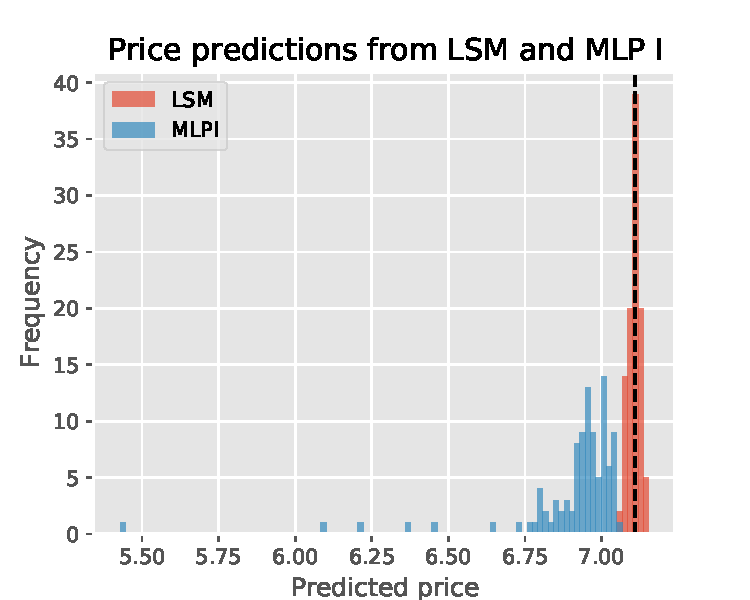
\includegraphics{Figures/histLSMMLPsI.pdf}
\decoRule
\caption[Price Predictions Histogram]{100 predicted prices for American put option with LSM and MLP I. Parameters are T=1, $\sigma=0.4$, $r=0.06$, $S(0)=36$, and $K=40$. Note CRR price is the dashed black line.}
\label{fig:histLSMMLPI}
\end{figure}

Improvements of MLP I is needed in order for the method to challenge the existing LSM, both in terms of speed and accuracy for low dimensional problems. Possible improvement of the MLP I could be conducted by a large hyperparameter tuning study. The issue with hyperparameter tuning is that it is computationally expensive. For the MLP I the hyperparameter tuning needs to be searched at every exercise date. Another type of network could also be considered, e.g. recurrent neural network. The inferior results from the MLP I to the LSM show that some work still needs to be done. We choose not to consider MLP I and LSM for the next section, because of the poor results from the MLP I pricing method in this section.
%----------------------------------------------------------------------------------------
%	SECTION 3
%----------------------------------------------------------------------------------------
\section{American Put Minimum on two Assets Option}\label{bivariateAmerPut}
There are many exotic American options to consider, but we choose to focus on the American put minimum on two stocks option, because MLP II is trained to predict prices on this specific option. The other advantage is that we have the deterministic method BEG for the bivariate contingent claim, hence, the MLP II can easily be compared, both for accuracy and speed.\\

First, we look at the computational cost for the BEG model by increasing the number of time-steps. By looking at table \ref{tab:TradeOffAmerMin} it is clear that the computational time is dependent on the number of time-steps. We know from the discussion in section \ref{EuroOption} that the accuracy increases by increasing the number of time-steps. Weighing the computational cost and accuracy, we choose to use the BEG pricing model as reference price with 500 time-steps. Note that when we generated the labels for the MLP II pricing method, we used 50 equidistant time-steps. The reason for using 50 time-steps is that we simulated 300.000 data points, which is a computationally heavy task. A MLP II model trained with 500 time-steps would probably predict the price from the BEG model with 500 steps better, but it was not computationally feasible. This creates an expectation that the option priced with MLP II will have a bias price and therefore, we will also include the BEG with 50 time-steps in the comparison.\\

\begin{table}[th]
\caption{BEG for the American Bivariate Contingent Claim}{Comparison of speed for the American put minimum on two assets option, where the inputs are K=40, $S_1(0)=S_2(0)=40$, $\sigma_1=0.2, \sigma_2=0.3$, T=1, $\rho=0.5$  and r=0.06. Note ms is shorthand for millisecond}
\label{tab:TradeOffAmerMin}
\centering
\begin{tabular}{l l l l}
\toprule
\textbf{Method} & \textbf{No. Steps} & \textbf{Price} & \textbf{Time: min:sec.ms} \\
\midrule
BEG & 10 & 4.524 & 00:00.006\\
& 50 & 4.594 & 00:00.250\\
& 100 & 4.602 & 00:01.837\\
& 200 & 4.605 & 00:14.025\\
& 500 & 4.608 & 03:35.039\\
& 1000 & 4.609 & 28:32.584\\
MLP II &  & 4.426 & 00:00.0003\\
\bottomrule\\
\end{tabular}
\end{table}

Table \ref{tab:TradeOffAmerMin} shows that the price for the American put minimum is greater than the European put minimum from table \ref{tab:TradeOffEuroMin}. Additionally, it is clear that the computational time increases for the American option, because we have to compare intrinsic value and expected continuation value at each node. Both results are good sanity checks.\\

For visualization we plot the BEG50, BEG500, and MLP II for varying spots with fixed K=40, $\sigma_1=0.2$, $\sigma_2=0.3$, T=1, $\rho=0.5$,  and r=0.06. The figure shows that the BEG500\footnote{BEG model with 500 time-steps} and BEG50 are close to each other. The total absolute deviation is 0.142 for the 21 prices, which shows that the BEG50 is sufficient for training our MLP. The total absolute deviation for the MLP II with the BEG500 is 3.716 and with the BEG50 3.713. This is depicted in figure \ref{fig:BEGMLPII}, where the MLP underprices the option for the in-sample domain with varying spot. To compare the computational speed the MLP II took around 00:00.000349 to generate one price, which is considerably faster than the BEG model with 10 time-steps. Hence, we see that we loose some accuracy with the MLP II, but the pricing method is fast. \\

\begin{figure}[H]
\centering
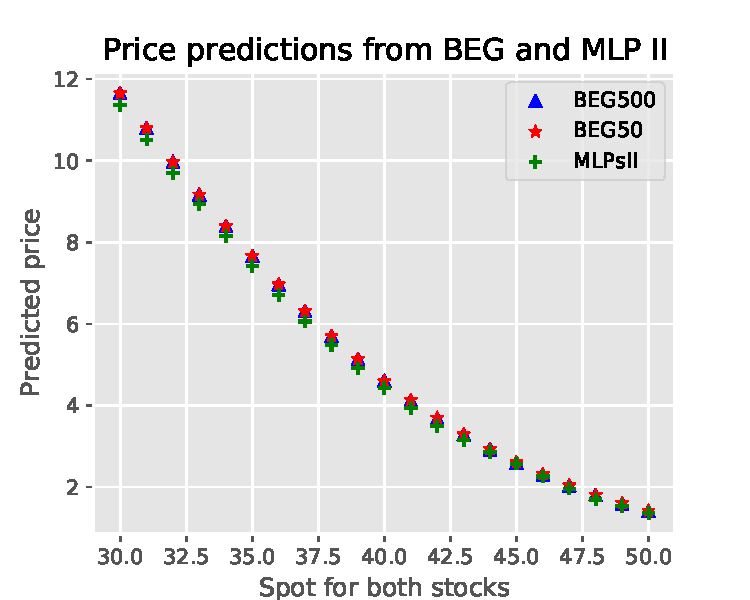
\includegraphics{Figures/compareBEGMLPsII.pdf}
\decoRule
\caption[Compare BEG and MLP II]{Scatter plot of predicted prices for American put minimum on two assets option with BEG and MLP II. Parameters are T=1, $\sigma_1=0.2$, $\sigma_2=0.3$, $r=0.06$, $K=40$ and $\rho=0.5$. Note BEG is showed for 50 time-steps and 500 time-steps.}
\label{fig:BEGMLPII}
\end{figure}

The MLP might provide a better estimate by simulating more data samples and make the model more complex, but our hyperparameter tuning study was not conclusive on this point. Hyperparameter tuning could also be further investigated, e.g. looking at depth and width of the network. The real power of pricing with MLP II is when the computational burden becomes an issue for fast pricing. 

%----------------------------------------------------------------------------------------
%	SECTION 4
%----------------------------------------------------------------------------------------
\section{Discussion of Pricing Methods}
The idea behind using neural networks instead of the linear model, is that the neural networks scale better for high dimensional problems. We have only considered univariate and bivariate contingent claims because in these cases, we have a deterministic alternative in the binomial lattice models. This gives a good indication of how the model predicts. Besides, if the model does not perform well for low dimensional problems, we would not expect the model to be any better for more complex multivariate contingent claims.\\

Remember, the binomial lattice model also has its limitations in terms of computational resources, because the computational burden scales exponentially with the number of underlying risky assets\footnote{The same can be said about the PDE methods}. The LSM is versatile and can be used for most derivatives, because it relies on Monte Carlo simulation and regression. For considering multivariate contingent claims the LSM is readily useful, but the linear model for regression suffers the curse of dimensionality for basket options with many underlying risky assets. We have in mind that a neural network does not suffer from the curse of dimensionality, hence the method, compared to the linear model, has advantages when considering multivariate contingent claims. The idea of neural network should work in theory\footnote{Universal approximation theorem for MLP}, but the numerical results shown in this chapter are not satisfying for the MLP I in the univariate case.\\

The MLP II is somewhat better, but it still relies on existing option pricing methods or real market data. Therefore, it does not solve the curse of dimensionality for basket options with many underlying assets. The MLP II however, has the advantage of the increased speed after training, which could be beneficial in some circumstances. The MLP II could also be used on real data and it is versatile enough to capture the volatility shew\footnote{Explanation below in section "Discussion of the Black-Scholes model"} for equity options. One drawback is that there should be enough data samples, which is relevant if the method is used on real market data. Another drawback is that the trained model would need to be calibrated regularly, because financial scenarios can change dramatically, e.g. the financial crisis in 2007-2009.\\

In the training phase of the neural networks the derivatives of the model parameters are used for minimizing the cost function. The derivatives are calculated efficiently with back propagation, which is important for risk management. Potentially, the neural networks can speed up the risk management of the derivative books and give real time risks. Deep learning for risk management is investigated in \parencite{AntoineSavine}. It should be mentioned, that the above-mentioned methods cannot only be used for equity options, the LSM is e.g. widely used for fixed income\footnote{E.g. Libor Market Model}.\\

The results from the MLP I were a bit discouraging, because it was inferior to the LSM. The computational cost is higher for the MLP I for low dimensional problems, hence, an accuracy on the same level as for the LSM would make it attractive to investigate for higher dimensional problems. One explanation could be wrong hyperparameters for the model, which would require a time consuming hyperparameter search. The grid search might have its shortcomings in this aspect, because it requires some knowledge about possible well-suited hyperparameters for the optimal stopping problem. A random search or Bayesian search could be beneficial in this aspect, but it would also require many computational resources.\\

The MLP II lack some precision compared to LSM for the univariate contingent claim. For the bivariate the MLP II again showed a loss of accuracy, but showed additional speed. A larger hyperparameter study could also be conducted here, a different method to generate labels or a bigger data set could have been sampled. E.g. the article \parencite{FergusonRyan2018} shows good results for an European basket option with 6 underlying assets by simulating a data set of 500M samples. 

%----------------------------------------------------------------------------------------
%	SECTION 5
%----------------------------------------------------------------------------------------
\section{Discussion of the Black-Scholes model}
For pricing we utilize the Black-Scholes theory, where we assume constant volatility, the interest rate is constant through time, and future stock prices are lognormal distributed. It is well-known that the volatility is not constant, in fact, it depends on the maturity and strike. The dependency on strike and maturity can be modeled with a volatility surface. Looking only at one dependency the implied volatility for equity options is a decreasing function of the strike over spot $\frac{K}{S(0)}$ for real data (p. 458 \parencite{Hull}). This phenomenon is known as volatility shew for equity options. \\

A possible reason for the volatility shew is that investors are more concerned with falling stock prices than rising prices, hence, the volatility is instantaneously negatively correlated with the stock price. To overcome the issue about assuming constant volatility, a model with stochastic variance can be considered. The model becomes more complex with an extra stochastic variable, where for simplicity we mention the two factor Heston model. The basic model is given by the stock follow the SDE:
$$dS(t)=\alpha S(t) dt + \sqrt{V(t)} S(t) dW_S(t)$$
And the stochastic variance process $V(t)$ is the solution to the SDE:
$$dV(t)=a(\theta - V(t))dt + \epsilon \sqrt{V(t)} dW_V(t) \quad where \ a>0,\theta>0, \epsilon>0, \ and \ V(0)>0$$
Where $W_S(t)$ and $W_V(t)$ have correlation $\rho$. The interpretation of the constants is:
\begin{enumerate}
\item[•] $\theta$ is the long run average price variance
\item[•] a is the rate which $V(t)$ reverts to $\theta$
\item[•] $\epsilon$ is the volatility of the volatility
\end{enumerate} 
The implication of $\epsilon$ is that $V(t)$ is more volatile when volatility is high. The correlation between the stock and variance process is often modeled with a negative correlation. The negative correlation between the two processes displays the real market phenomenon of volatility shew for equity options, because when the stock price drops, volatility increases. Assuming stochastic volatility the Heston model overcomes the issue with volatility shew. Another model trying to solve the non-constant volatility is e.g. \textsl{"Constant Elasticity of Variance model"}, but there are numerous others\footnote{E.g \textsl{"Merton's Mixed Jump-Diffusion Model"} and \textsl{"Variance-Gamma Model"}}. \\

The constant risk-free interest rate through time assumption can also be discussed, because the interest rate is not constant for real market behavior. We did not investigate the American call, because it coincides with the European call for positive interest rate. Today's market interest rates are negative for the Eurozone, which was probably unheard before the last decade's financial events. Therefore, the decision to assume positive constant interest rate through time is set for convenience.\\

The Black-Scholes model assumes that the underlying risky assets evolve as a GBM, where the distribution of possible stock prices at the end of any interval is lognormal. The model is convenient, because the GBM has a analytical solution\footnote{SDE does not always have a analytical solution}. If we wanted to investigate arithmetic mean basket option the Bachelier model would be more convenient, because the future stock price is normal distributed. 
\begin{equation*}
dS_i=\sigma_i dW_i
\end{equation*}
This assumption would simplify the pricing problem of arithmetic basket options, because the sum of normal random variables provides a multivariate normal distribution. The pricing problem of the basket option in the Bachelier is then essentially one-dimensional. This is similar to the the geometric mean basket option for the Black-Scholes model (section \ref{GeoBasket}). A disadvantage with the Bachelier model is that it can lead to negative stock values, which is not realistic.\\

The Black-Scholes model has some drawbacks where you can question the assumptions, but the model is convenient to use for comparison of pricing methods. By the above discussion, we stress that we do not necessarily believe that the Black-Scholes model is the true model for real market behavior. The purpose is rather to investigate pricing methods in a convenient model.

